\section{Stoffklassen}

\small{\begin{tabularx}{\columnwidth}{|l|l|l|X|}
	\hline
	\textbf{Stoffklasse} & \textbf{Bindungstyp} & \textbf{Beispiel} & \textbf{Eigenschaften} \\
	\hline
	Salze & Ionenbindung & NaCl, CaCl\textsubscript{2} & Spröde, \newline hohe Schmelzpunkte, lösen sich oft gut in Wasser \\
	\hline
	Metalle & Metallbindung & Cu, Fe, Al & Leitfähig, glänzend \\
	\hline
	Molekulare Stoffe & Kovalente Bindung & H\textsubscript{2}O, CO\textsubscript{2}, CH\textsubscript{4} & niedrige Schmelz- und Siedepunkte, oft gasförmig oder flüchtig \\
	\hline
\end{tabularx}}

\subsection{Bindungen}

\subsubsection{Elektronenpaar-Bindung}

Dieser Bindungstyp existiert ausschließlich bei \textbf{Nichtmetall}-Atomenverbänden. \newline Diese Atomverbände sind meist \textbf{Moleküle} (mit begrenzter Atom-Anzahl).

\textbf{Beispiele:} H\textsubscript{2}O, C\textsubscript{2}H\textsubscript{6} (Ethan), C\textsubscript{2}H\textsubscript{5}OH (Ethanol), NH\textsubscript{3} (Ammoniak)

\subsubsection{Metall-Bindung}

Dieser Bindungstyp tritt auf, wenn ausschließlich \textbf{Metall}-Atome den Atomverband bilden. Dieser besteht aus einem \textbf{Metallgitter} aus ``unendlich'' vielen Atomen.

\textbf{Beispiele:} Pb (Blei), Cu (Kupfer), Ag (Silber), Na (Natrium), Mg (Magnesium), Pd (Palladium)

\subsubsection{Ionen-Bindung}

Dieser Bindungstyp entsteht immer, wenn \textbf{Nichtmetall}-Atome mit \textbf{Metall}-Atomen reagiert haben. Er hält die bei der Reaktion gebildeten Ionen in einem Gitter aus ``unendlich'' vielen Ionen zusammen (= \textbf{Ionengitter}).

\textbf{Beispiele:} Na\textsuperscript{+}Cl\textsuperscript{--} (Natriumchlorid), Mg\textsuperscript{2+}Cl\textsubscript{2}\textsuperscript{--} (Magnesiumchlorid), K\textsuperscript{+}I\textsuperscript{--} (Kaliumiodid)


\subsection{Bindungswinkel}
\begin{center}
	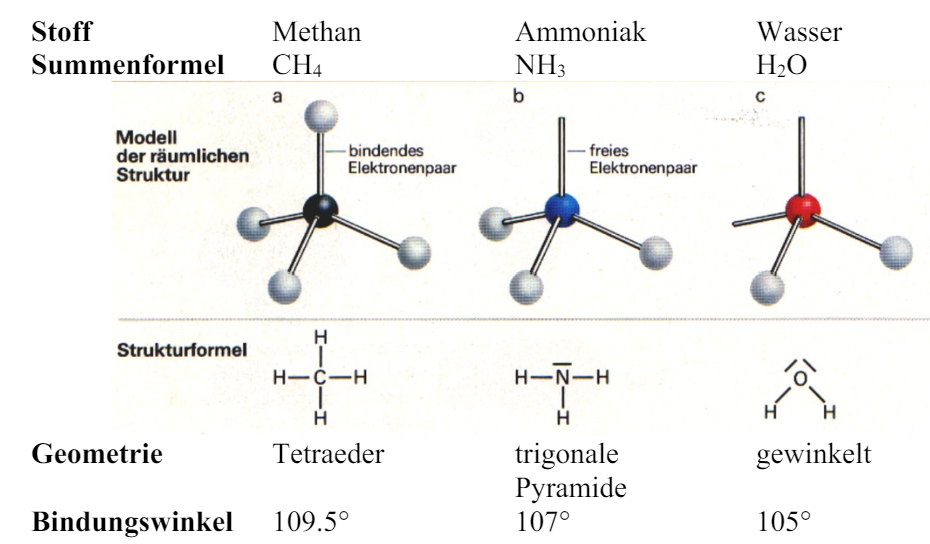
\includegraphics[height=4cm]{images/Winkel.png}
\end{center}

\subsection{Metalle und Halbmetalle}
 $\rightarrow$ Metalle besitzen durch delokalisierte Elektronenwolken (VE) dh. freie Ladungsträger, dies führt zu gute Wärme- und el. Leitfähigkeit, Verformbarkeit
\subsubsection {Leitfähigkeit bei Metallen}
	\begin{itemize}
		\item nimmt mit steigender Temperatur ab
		\item die Bewegung der Atomrümpfe erhöht sich
		\item weniger Platz für die Elektronenbewegung
	\end{itemize}
	
\begin{minipage}{0.48\columnwidth}
	\textbf{Beispiel Lithium:}
	\begin{itemize}
		\item Valenzband Vb nicht ganz gefüllt
		$\rightarrow$ Elektronen können sich im Band bewegen
	\end{itemize}
\end{minipage}
 \hfill
\begin{minipage}{0.48\columnwidth}
	\textbf{Beispiel Beryllium:}
	\begin{itemize}
		\item Valenzband komplett gefüllt, aber mit leerem Leitungsband überlappend
		$\rightarrow$ Elektronen können sich im Band bewegen
	\end{itemize} 
\end{minipage}
\begin{center}
	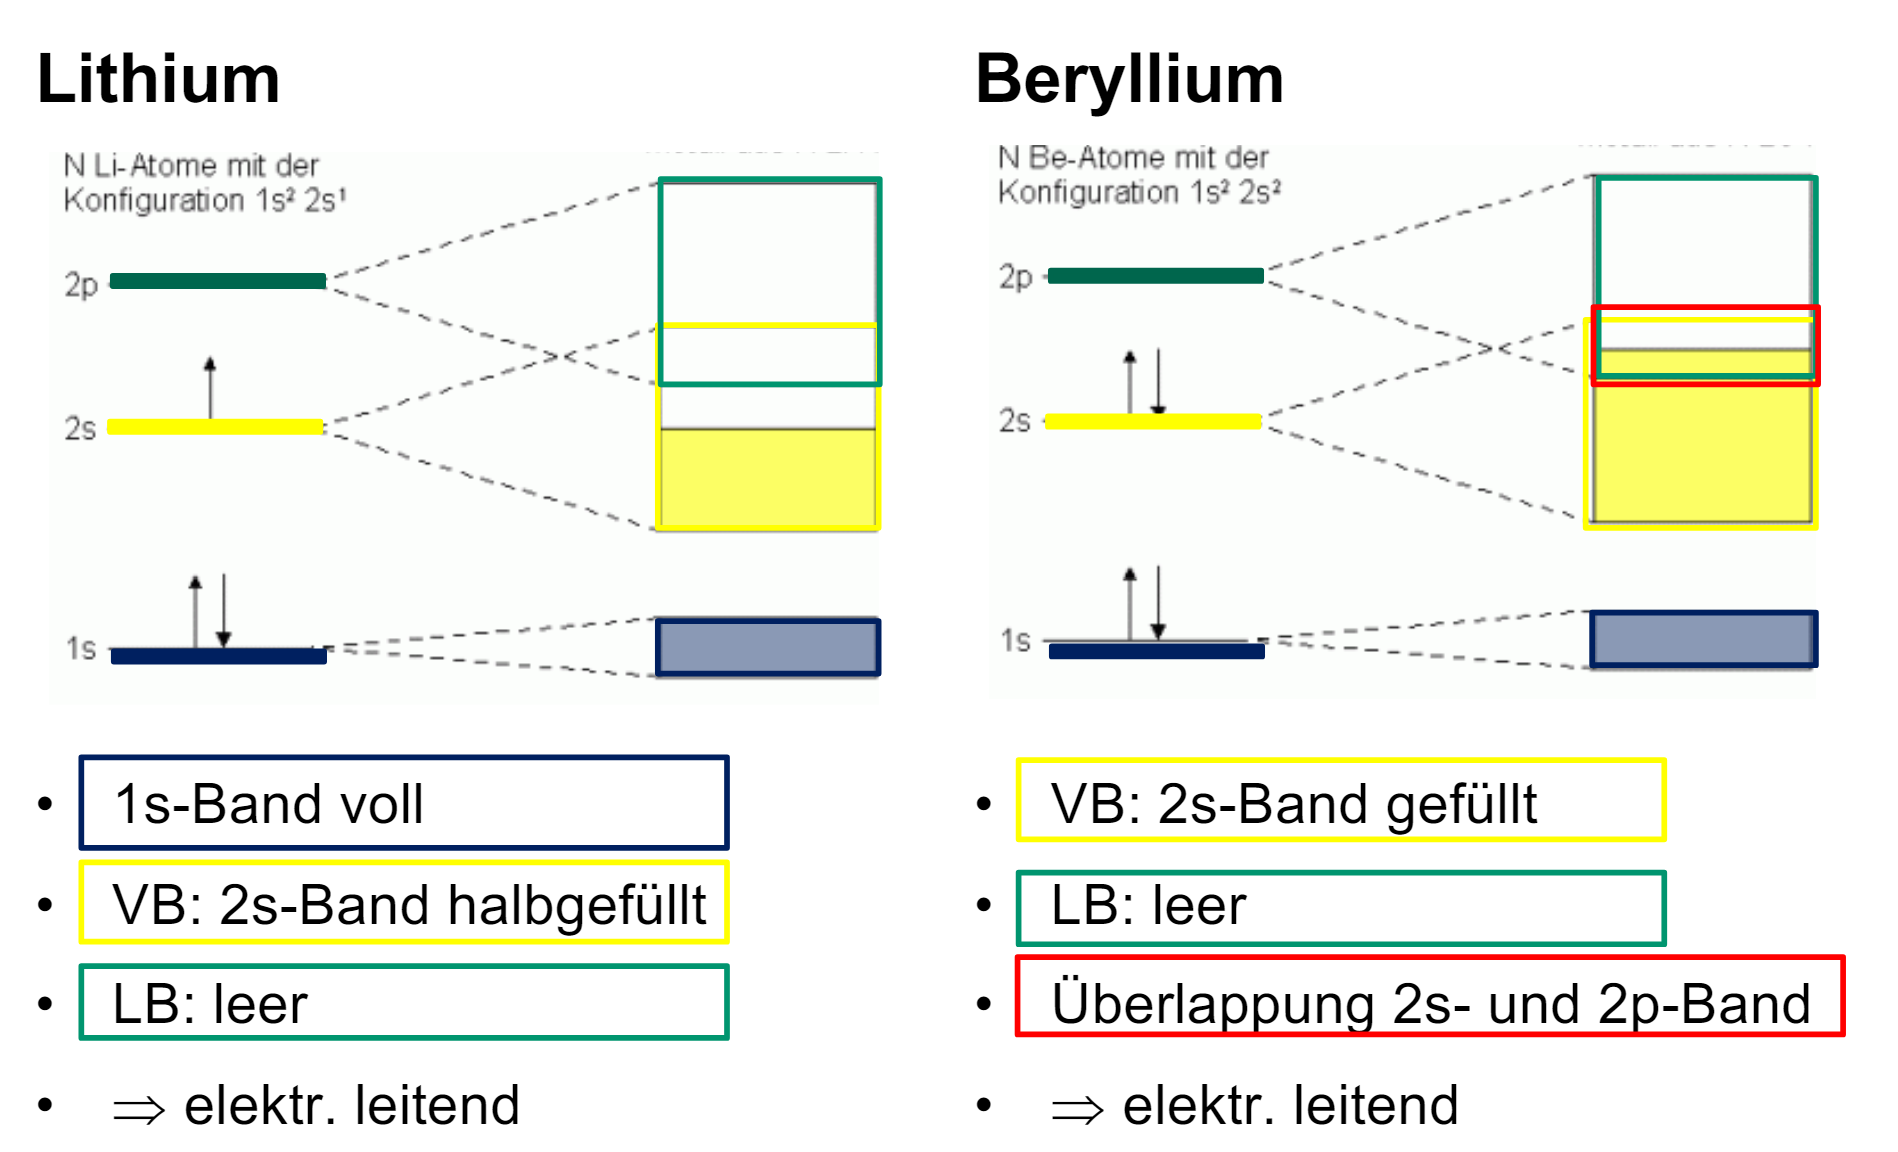
\includegraphics[height=3cm]{images/Baender.png}
\end{center}

 $\rightarrow$ Halbmetalle haben weder Elektronenwolken noch überlappende Energieniveaus, Nähe vom Valenz- und Leitungsband ermöglichen aber ein Überspringen
\subsubsection{Leitfähigkeit bei Halbmetallen}
	\begin{itemize}
		\item nimmt mit steigender Temperatur stark zu
		\item die Elektronen springen viel zahlreicher auf das Leitungband über
		\item Platz für Elektronenbewegung im Leitungsband
	\end{itemize}
	
\subsection{Dotierung von Halbmetallen}
Dotierung $\rightarrow$ Einbringen von Fremdatomen ins Atomgitter eines Halbleiters
\begin{itemize}
	\item \textbf{n-Halbleiter}
	\item[] z.B. einzelne As-Atome im Si-Gitter(1:10'000'000)
	\item[] Ein \tikz[baseline=(text.base)]\node[fill=orange, fill opacity=0.3, text opacity=1, rounded corners, inner sep=2pt, minimum height=5pt] (text) {\textit{überschüssiges}}; 
	Elektron pro As-Atom $\Rightarrow$ Leitfähigkeit: Elektron von As-Atom kann ins Leitungsband von Si überspringen und sich frei bewegen
	\item \textbf{p-Halbleiter}
	\item[] z.B. einzelne B-Atome im Si-Gitter(1:1'000'000)
	\item[] Ein \tikz[baseline=(text.base)]\node[fill=orange, fill opacity=0.3, text opacity=1, rounded corners, inner sep=2pt, minimum height=5pt] (text) {\textit{fehlendes}}; Elektron pro B-Atom $\Rightarrow$ Leitfähigkeit: Elektronen aus dem vollen Valenzband von Si können in diese ``Lücke'' springen und sich frei bewegen
\end{itemize}
